% bayanihan-net -- consolidation deck for the grader.
% Compiles with pdflatex (run twice). Numbers are the committed, post-fix canonical values;
% the source of truth for every figure is evidence/*.json (see the paper and docs for detail).
\documentclass[aspectratio=169,11pt]{beamer}
\usetheme{Madrid}
\usecolortheme{whale}
\setbeamertemplate{navigation symbols}{}
\setbeamertemplate{caption}[numbered]
\usepackage{booktabs}
\usepackage{amsmath}
\usepackage{tikz}
\usetikzlibrary{arrows.meta, positioning}
\usepackage{xcolor}

\setbeamertemplate{frametitle continuation}{}
\setbeamercolor{block title}{bg=structure.fg!18,fg=black}
\setbeamercolor{block body}{bg=structure.fg!6}
\newcommand{\sig}{$^{\star}$}

\title[bayanihan-net]{\textbf{bayanihan-net}}
\subtitle{A hybrid multi-agent system for disaster-response coordination under scarcity}
\author[Capstone]{Designing \& Building Agentic AI Systems --- Capstone}
\institute[McGill MMA]{Marikina flood basin, Metro Manila \quad$\cdot$\quad reproducible from seed \texttt{20260620}}
\date{}

\begin{document}

\begin{frame}[plain]
  \titlepage
  \begin{center}\footnotesize
  A consolidation of the repo's README, eight design docs, and the arXiv-style paper.\\
  Graded on the working code; every number below regenerates from a seed with no API key.
  \end{center}
\end{frame}

\begin{frame}{Roadmap}
  \small
  \begin{columns}[T]
    \column{0.5\textwidth}
    \begin{enumerate}
      \item The problem (system brief)
      \item Why MAS --- a single agent is not enough
      \item Architecture
      \item Agent roster
      \item Communication contract
      \item Coordination --- a defended hybrid
    \end{enumerate}
    \column{0.5\textwidth}
    \begin{enumerate}\setcounter{enumi}{6}
      \item Incentives \& emergence
      \item Interoperability (MCP / A2A)
      \item Prototype \& simulation
      \item Evaluation (four levels, honest result)
      \item Safety \& governance
      \item MARL bridge \& reflection
    \end{enumerate}
  \end{columns}
\end{frame}

% ---------------------------------------------------------------- problem
\begin{frame}{1 \;\; The problem --- a Marikina typhoon flood}
  \small
  A typhoon stalls over Metro Manila; the Marikina River rises through its alarm levels and
  six low-lying barangays flood within hours. The city disaster office (CDRRMC) must allocate
  a \textbf{small fleet of scarce assets} across many simultaneous, evolving incidents.
  \begin{columns}[T]
    \column{0.54\textwidth}
    \textbf{Stakeholders \& stakes}
    \begin{itemize}\small
      \item $\sim$5{,}100 residents at risk across 6 barangays
      \item 9 assets: 4 boats, 3 trucks, 2 medical teams
      \item Duty officer holds authority over irreversible calls
      \item Partner agencies (mutual aid); upstream feeds (PAGASA/MMDA/DOH)
    \end{itemize}
    \column{0.46\textwidth}
    \textbf{Why it is hard}
    \begin{itemize}\small
      \item Scarcity is binding (capacity-saturated)
      \item Irreversibility (a crew on-scene cannot be un-sent)
      \item Partial observability \& degradation
      \item Adversarial / noisy citizen reports (Sybil)
    \end{itemize}
  \end{columns}
  \vspace{0.4em}
  \begin{block}{Objective}
    Minimize total \textbf{severity-weighted unmet need}, equitably and safely, under hard
    asset scarcity. \footnotesize(Geography/figures are illustrative stand-ins, not official data.)
  \end{block}
\end{frame}

% ---------------------------------------------------------------- why MAS
\begin{frame}{2 \;\; Why a multi-agent system --- a single agent is the wrong shape}
  \small
  \begin{enumerate}
    \item \textbf{Partial observability.} No vantage sees the whole flood --- scouts, the river
      gauge, and citizen reports each see a slice; the truth is \emph{assembled}.
    \item \textbf{Specialized expertise.} Triage, mass-casualty judgement, logistics, routing
      under flooding, and hydrology are different competencies with different state and tools.
    \item \textbf{Parallel decomposition.} Many concurrent incidents; a single agent serializes.
    \item \textbf{Resilience / graceful degradation.} A typhoon degrades power and comms ---
      a single point of control is a single point of failure, fatal in disaster response.
    \item \textbf{Organizational alignment.} Real response \emph{is} multi-agency:
      barangay $\rightarrow$ city $\rightarrow$ NDRRMC, plus relief, health, rescue, NGOs.
  \end{enumerate}
  \vspace{0.3em}
  \footnotesize We adopt MAS because the \emph{problem} is distributed, specialized, concurrent,
  failure-prone, and inter-organizational --- not because MAS is fashionable.
\end{frame}

% ---------------------------------------------------------------- architecture
\begin{frame}{3 \;\; Architecture}
  \centering
  \resizebox{\textwidth}{!}{%
  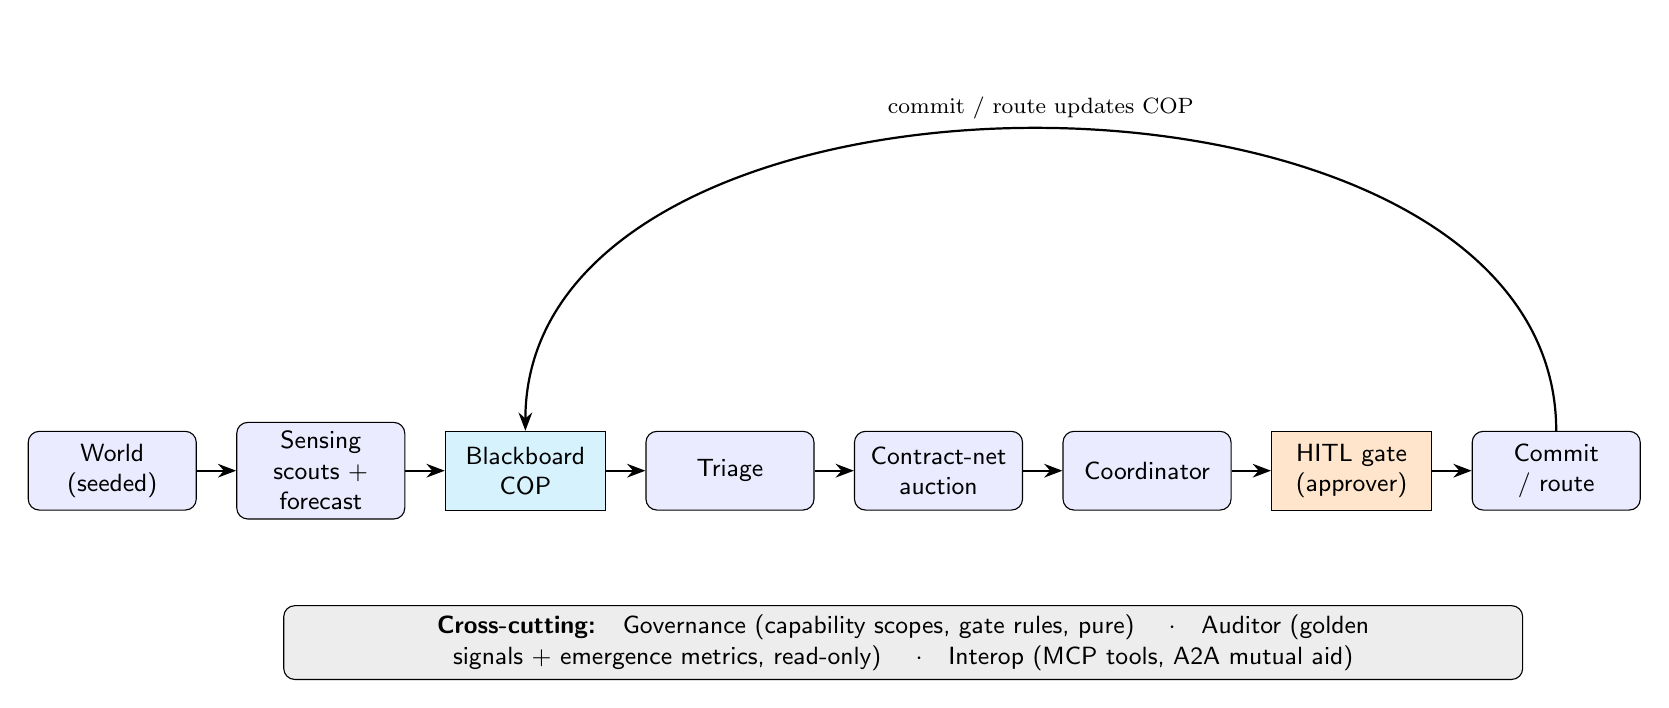
\begin{tikzpicture}[font=\sffamily\small, >=Stealth, node distance=0.5cm,
    box/.style={draw, rounded corners, align=center, minimum height=1cm, text width=1.9cm, fill=blue!8},
    cop/.style={draw, align=center, minimum height=1cm, text width=1.8cm, fill=cyan!16},
    gate/.style={draw, align=center, minimum height=1cm, text width=1.8cm, fill=orange!20}]
    \node[box] (w) {World (seeded)};
    \node[box, right=of w] (s) {Sensing scouts + forecast};
    \node[cop, right=of s] (c) {Blackboard COP};
    \node[box, right=of c] (t) {Triage};
    \node[box, right=of t] (a) {Contract-net auction};
    \node[box, right=of a] (co) {Coordinator};
    \node[gate, right=of co] (g) {HITL gate (approver)};
    \node[box, right=of g] (o) {Commit / route};
    \foreach \x/\y in {w/s,s/c,c/t,t/a,a/co,co/g,g/o} \draw[->, thick] (\x)--(\y);
    \draw[->, thick] (o) to[out=90,in=90] node[above,font=\footnotesize]{commit / route updates COP} (c);
    \node[draw, rounded corners, fill=gray!14, below=1.2cm of t, text width=15.5cm, align=center, xshift=2.2cm]
      {\textbf{Cross-cutting:}\;\; Governance (capability scopes, gate rules, pure)
       \quad$\cdot$\quad Auditor (golden signals + emergence metrics, read-only)
       \quad$\cdot$\quad Interop (MCP tools, A2A mutual aid)};
  \end{tikzpicture}}
  \vspace{0.5em}\\
  \footnotesize Each tick: world advances $\rightarrow$ COP refreshes $\rightarrow$ triage prioritizes
  $\rightarrow$ auction $\rightarrow$ award (through the HITL gate) $\rightarrow$ assets move along
  risk-aware routes, \emph{validated against the true flood at arrival}. The control plane is pure,
  deterministic Python; only the world is stochastic (one seed).
\end{frame}

% ---------------------------------------------------------------- roster
\begin{frame}{4 \;\; Agent roster --- roles, scopes, escalation (enforced in code)}
  \scriptsize
  \begin{tabular}{@{}p{2.3cm}p{6.4cm}p{4.2cm}@{}}
    \toprule
    \textbf{Agent} & \textbf{Responsibility} & \textbf{Scopes / escalates} \\
    \midrule
    Sensing scout $\times$2 & citizen reports $\rightarrow$ COP incidents; flag Sybil & \texttt{cop:write} \\
    Hydromet / forecast & post river level (PAGASA gauge via MCP) & \texttt{cop:write, tool:pagasa.read} \\
    Triage & prioritize, dedupe, suppress uncorroborated Sybil; announce tasks & \texttt{taskboard:write} \\
    Logistics $\times$2 & own \& bid scarce assets (rescue boats / relief trucks) & \texttt{asset:bid, asset:commit} \\
    Medical & bid teams; watch mass-casualty overload & \texttt{+escalation:raise} (edge-triggered) \\
    Routing & risk-aware routes over a \emph{belief} of the flood & \texttt{tool:mmda.read} (advises) \\
    Coordinator & re-score on welfare, award, gate, atomic commit, rollback & \texttt{asset:award, rollback:issue} \\
    Human approver & approve/deny irreversible commits from a decision package & final authority \\
    Auditor & read-only: outcome + emergence reports & \texttt{audit:read} \\
    \bottomrule
  \end{tabular}
  \vspace{0.4em}\\
  \footnotesize Memory is \textbf{externalized}: the durable store is the COP + append-only event log,
  not hidden per-agent state. Boundaries are enforced --- every COP write is gated at the bus on the
  sender's \texttt{cop:write} scope.
\end{frame}

% ---------------------------------------------------------------- comms
\begin{frame}{5 \;\; Communication contract}
  \small
  \begin{columns}[T]
    \column{0.52\textwidth}
    \textbf{Typed envelope} (Pydantic, \texttt{extra="forbid"})
    \begin{itemize}\footnotesize
      \item \texttt{schema\_version, trace\_id, message\_id}
      \item \texttt{correlation\_id, idempotency\_key, priority}
      \item \texttt{tick, deadline\_tick, security\_context, payload}
    \end{itemize}
    \texttt{message\_id} is deterministic (\texttt{agent:tick:seq:type}) --- \textbf{no uuid4}, so a
    seed replays the exact message sequence. 12 message verbs; a test asserts every verb has a payload.
    \column{0.48\textwidth}
    \textbf{Routing}
    \begin{itemize}\footnotesize
      \item pub/sub on the blackboard (observations)
      \item directed contract-net (CFP $\rightarrow$ bid $\rightarrow$ award)
      \item dedicated escalation channel (no-drop path)
    \end{itemize}
    \textbf{Shared state}
    \begin{itemize}\footnotesize
      \item idempotency, two layers (transport + content-key fusion)
      \item leases / freshness (stale-COP guard)
      \item atomic \texttt{try\_commit} (the no-double-commit chokepoint)
    \end{itemize}
  \end{columns}
  \vspace{0.3em}
  \footnotesize The MAS failure catalogue (deadlock, message storm, duplicates, stale state) is mapped
  row-by-row to a mitigation; lossy comms and Sybil are handled as domain threats.
\end{frame}

% ---------------------------------------------------------------- coordination
\begin{frame}{6 \;\; Coordination --- a defended hybrid}
  \small
  \begin{block}{The mechanism}
    \textbf{Blackboard} (shared COP) $+$ \textbf{contract-net} (scarce-asset auction) $+$
    \textbf{supervisor with HITL} (accountable arbitration \& escalation). Each leg is the right
    primitive for one sub-problem.
  \end{block}
  \textbf{Why not a pure mechanism} (each option on the course's coordination menu was considered):
  \begin{itemize}\footnotesize
    \item \emph{Pure supervisor} --- a single point of failure (fatal here) and a bottleneck.
    \item \emph{Pure market / contract-net} --- efficient allocation but \emph{no shared awareness}
      and no accountable escalation.
    \item \emph{Pure consensus} --- too slow and expensive for time-critical life-safety decisions.
    \item \emph{Pure blackboard} --- shared awareness but \emph{no decision-maker}.
  \end{itemize}
  The hybrid composes all three: shared awareness \emph{and} efficient allocation \emph{and}
  accountable escalation --- and it \textbf{degrades gracefully} (lose the coordinator $\rightarrow$
  agents fall back on the last-known COP).
\end{frame}

% ---------------------------------------------------------------- incentives + emergence
\begin{frame}{7 \;\; Incentives \& emergence}
  \small
  \begin{columns}[T]
    \column{0.5\textwidth}
    \textbf{Incentives --- local vs.\ global}\\
    Each logistics agent locally wants its own utilization; the global goal is to minimize
    severity-weighted harm. Resolved \emph{structurally}: \textbf{the bidder does not choose the winner}.
    The coordinator ranks on a global welfare score
    \[\footnotesize W=\frac{\text{sev}\cdot\min(\text{cap},\text{ppl})}{\text{eta}+1}\Bigl(1-\tfrac12\,\text{risk}\Bigr)\]
    so hoarding or cherry-picking cannot win --- the welfare-maximizing (VCG-flavoured, no payments)
    allocation rule.
    \column{0.5\textwidth}
    \textbf{Emergence --- named, with detector $\to$ guardrail}\\
    \footnotesize
    \emph{Useful:} bayanihan division of labour; adaptive routing; load spreading (entropy $\approx0.97$).\\[2pt]
    \emph{Unwanted:}
    \begin{itemize}
      \item oscillation $\to$ reassignment rate $\to$ hysteresis
      \item inequity $\to$ coverage Gini / worst-served $\to$ severity-first
      \item report-storm $\to$ Shannon entropy $\to$ content-key dedup
      \item stale-COP $\to$ freshness $\to$ leases + arrival validation
      \item over-escalation $\to$ rate $\to$ edge-triggered
    \end{itemize}
  \end{columns}
\end{frame}

% ---------------------------------------------------------------- interop
\begin{frame}{8 \;\; Interoperability --- MCP and A2A boundaries}
  \small
  Two distinct boundaries, both \textbf{real in code} with mocked upstreams.
  \begin{columns}[T]
    \column{0.5\textwidth}
    \textbf{MCP --- scoped tool/context}
    \begin{itemize}\footnotesize
      \item PAGASA river gauge: the \textbf{live} hop, invoked every tick (\textbf{48 traced calls/run})
      \item MMDA closures, DOH beds: \emph{registered \& scope-declared but not invoked}
      \item every adapter declares its scope; an under-scoped caller is refused (tested)
    \end{itemize}
    \column{0.5\textwidth}
    \textbf{A2A --- cross-org work exchange}
    \begin{itemize}\footnotesize
      \item medical mutual aid from a neighbouring agency (Quezon City CDRRMC)
      \item typed task; \textbf{local access policy owned by the receiver}
      \item idempotency + retry; trace propagation (1 request/run, completed)
    \end{itemize}
  \end{columns}
  \vspace{0.4em}
  \footnotesize The \emph{boundary and the policy gate} are real in code --- the part that matters for
  safety --- not an LLM tool-call layer; the upstream services are simulated.
\end{frame}

% ---------------------------------------------------------------- prototype
\begin{frame}{9 \;\; Prototype --- a deterministic, reproducible simulation}
  \small
  Discrete-event simulation over a \textbf{12-hour horizon} (48 ticks $\times$ 15 min), seed
  \texttt{20260620}. One \texttt{cli run} produces a full worked scenario and stamped evidence.
  \begin{columns}[T]
    \column{0.5\textwidth}
    \textbf{Committed evidence}
    \begin{itemize}\footnotesize
      \item \texttt{run\_log.txt} --- one incident, end to end
      \item \texttt{audit\_log.jsonl} --- immutable event spine
      \item \texttt{decision\_package.json} --- a real HITL package
      \item \texttt{scenario\_report.json} --- outcome + golden signals
      \item 5 figures (COP timeline, coverage, RL curve, \dots)
    \end{itemize}
    \column{0.5\textwidth}
    \textbf{Worked run (seed 20260620)}
    \begin{itemize}\footnotesize
      \item served \textbf{266 / 776} people (34.3\%)
      \item dispatch SLA 47.0\%; 1 escalation
      \item HITL: 12 approvals / 7 denials
      \item \textbf{byte-identical} on re-run; fingerprint \texttt{013f8d40ba7f}
    \end{itemize}
  \end{columns}
  \vspace{0.3em}
  \footnotesize Proven from a clean room: a fresh checkout + the README quickstart regenerates all 8
  evidence artifacts \emph{byte-for-byte}.
\end{frame}

% ---------------------------------------------------------------- evaluation
\begin{frame}{10 \;\; Evaluation --- four levels, and an honest result}
  \scriptsize
  Two tiers: \textbf{Tier A} invariants are a hard gate; \textbf{Tier B} is the comparative study
  (12 paired seeds, 5 ablation baselines, means $\pm$SE). A delta is flagged on a 2-SE \emph{screen}
  (not a $t$-test --- stated honestly). Every level emits real numbers (agent / interaction / system /
  human+emergence) plus the six MAS golden signals.
  \vspace{0.3em}
  \begin{columns}[T]
    \column{0.46\textwidth}
    \begin{tabular}{@{}lcc@{}}
      \toprule
      Policy & sev-wt served & worst-served \\
      \midrule
      \textbf{hybrid} & 0.353 & 0.220 \\
      no\_governance & 0.355 & 0.222 \\
      greedy\_nearest & 0.354 & 0.217 \\
      fifo & 0.348 & 0.220 \\
      fairness\_weighted & 0.350 & 0.212 \\
      random & 0.340 & 0.203 \\
      \bottomrule
    \end{tabular}
    \column{0.54\textwidth}
    \textbf{What the data supports (honestly):}
    \begin{itemize}
      \item The \emph{only} paired-significant service gain is \textbf{hybrid $>$ random}
        (sev-wt $+0.0125$\sig, raw served $+0.0136$\sig): you need triage + welfare scoring.
      \item Against the other \emph{reasonable} policies (greedy, FIFO, fairness) the deltas are
        \textbf{within noise} --- under hard saturation, \emph{reachability and capacity bind, not the
        allocation rule}.
      \item The HITL gate costs a small, significant $-0.0086$\sig dispatch-SLA --- the reserve trade.
    \end{itemize}
  \end{columns}
  \vspace{0.2em}
  \footnotesize\sig\,$=$ clears the 2-SE screen. Coordination's value here is beating \emph{no}
  coordination, plus safety and graceful degradation under stress --- not a separation between heuristics.
\end{frame}

% ---------------------------------------------------------------- safety
\begin{frame}{11 \;\; Safety \& governance}
  \small
  \begin{columns}[T]
    \column{0.5\textwidth}
    \textbf{Human-in-the-loop}
    \begin{itemize}\footnotesize
      \item gated by explicit, auditable rules: last scarce reserve, large commit
        (forced-evacuation reason defined \& tested, not yet triggered)
      \item the human gets a \textbf{decision package} (context, options, recommendation, risk) --- not chatter
    \end{itemize}
    \textbf{Rollback}
    \begin{itemize}\footnotesize
      \item reverse a reversible award (lease reclaim); \textbf{never yank an on-scene crew}
        (guard enforced + tested)
    \end{itemize}
    \column{0.5\textwidth}
    \textbf{Audit \& abuse cases}
    \begin{itemize}\footnotesize
      \item immutable event log with \texttt{trace\_id}; read-only auditor
      \item red-team stress battery: \textbf{all 7 scenarios pass} with zero safety-invariant violations
      \item Sybil, report-storm, comms blackout, 25\% asset loss, gauge outage, compound crisis
    \end{itemize}
    \textbf{Stance}
    \begin{itemize}\footnotesize
      \item safety constraints are \emph{enforced, not learned}
    \end{itemize}
  \end{columns}
\end{frame}

% ---------------------------------------------------------------- MARL bridge
\begin{frame}{12 \;\; MARL bridge --- is multi-agent RL appropriate?}
  \small
  \begin{columns}[T]
    \column{0.46\textwidth}
    \textbf{Not} for the live system:
    \begin{itemize}\footnotesize
      \item non-stationarity (agents co-learning)
      \item contested reward (whose objective?)
      \item governance needs \emph{deterministic, auditable} decisions, not a black box
    \end{itemize}
    \textbf{Yes}, offline, for routing: sequential, repeated, simulatable, delayed-reward.
    \column{0.54\textwidth}
    \textbf{The study} (tabular Q-learning, numpy; CTDE via parameter sharing) reproduces
    \textbf{reward hacking} --- the Assignment 2 bridge:
    \begin{center}\footnotesize
    \begin{tabular}{@{}lcc@{}}
      \toprule
      policy & true return & flood exposure \\
      \midrule
      \textbf{risk-aware (RL)} & \textbf{2.71} & \textbf{0.617} \\
      naive (RL) & 2.53 & 0.650 \\
      heuristic & 2.36 & 0.674 \\
      \bottomrule
    \end{tabular}
    \end{center}
    The naive (travel-time proxy) reward loses on the \emph{true} objective; the learned risk-aware
    policy even beats the heuristic. \textbf{Advisory only} --- the heuristic remains the authority.
  \end{columns}
\end{frame}

% ---------------------------------------------------------------- reflection
\begin{frame}{13 \;\; Reflection --- honest failures (the rubric rewards them)}
  \small
  \begin{itemize}
    \item \textbf{The fairness lever.} First a silent no-op (deficit scaled every bid equally), then
      ``backfiring,'' then --- after fixing a measurement bug --- \emph{within noise}. Kept as an
      evaluated, documented negative rather than deleted.
    \item \textbf{A served-count bug, caught and corrected.} The read-only auditor double-credited
      ``lives served'' when two genuine incidents fused at the COP. Fixing it \emph{lowered} the
      headline numbers and collapsed most significance --- we report the corrected, weaker result
      rather than the flattering one.
    \item \textbf{The capacity-bound finding.} In a saturated flood the binding constraint is
      \emph{which barangays you can reach with the assets you have}, not the allocation rule ---
      so the reasonable policies are statistically indistinguishable. That null \emph{is} the finding.
  \end{itemize}
  \vspace{0.2em}
  \footnotesize Honest failure analysis, not a victory lap --- the full build log is in
  \texttt{docs/REFLECTION.md}.
\end{frame}

% ---------------------------------------------------------------- close
\begin{frame}{14 \;\; The artifact --- reproducible end to end}
  \small
  \begin{columns}[T]
    \column{0.5\textwidth}
    \textbf{Engineering}
    \begin{itemize}\footnotesize
      \item 36 modules, acyclic DAG, complexity $\le 10$
      \item 55 behaviour/invariant tests, 98\% coverage
      \item ruff + mypy + markdownlint clean; deterministic
    \end{itemize}
    \textbf{Run it}
    \begin{itemize}\footnotesize
      \item \texttt{cli run / eval / stress / rl-train}
      \item \texttt{evals/run\_evals.py} --- Tier-A gate (non-zero exit)
    \end{itemize}
    \column{0.5\textwidth}
    \textbf{Where the detail lives}
    \begin{itemize}\footnotesize
      \item \texttt{README.md} --- narrative + rubric map
      \item \texttt{docs/} --- 8 design documents
      \item \texttt{paper/report.pdf} --- arXiv-style write-up
      \item \texttt{AGENTS.md} --- the roster contract
      \item \texttt{evidence/} --- every number traces here
    \end{itemize}
  \end{columns}
  \vspace{0.6em}
  \begin{block}{One-line defense}
    A small but credible MAS with a \emph{real} coordination mechanism, a \emph{real} safety story,
    and \emph{honest} failure analysis --- graded on behaviour, reproducible from a single seed.
  \end{block}
\end{frame}

\end{document}
